\documentclass{article}
\usepackage{fullpage}
\usepackage{amsmath}
\usepackage{amssymb}
\usepackage{amsfonts}
\usepackage{stmaryrd}
\usepackage{hyperref}
\usepackage[pdftex]{graphicx}

\title{Ray Tracing Cost: Checkpoint 2}
\author{Nicolas Feltman}
\begin{document}
\maketitle
\section{Progress}
The project has deviated slightly from the coarse set at the last checkpoint.  I spent a larger amout of time than anticipated building up a theoretical framework for describing ray intersection testing. Regardless, the project is on track to produce interesting results.

\subsection{Theory}
I have accomplished the following tasks in building up the theory of ray intersection testing:
\begin{itemize}
\item I described ray-box intersection in unambiguous mathematical terms.
\item I identified different kinds of culling for rays-box intersection.
\item I described the differences between traversal order schemes in terms of culling efficiency.
\item I isolated the cost of intersecting a distribution of rays with a BVH in simpler terms than previously existing in literature.
\item I rephrased top-down build effectiveness in terms of the true cost of a ray distribution.
\end{itemize}
\subsection{Tools}
I have accomplished the following tasks in development of tools.
\begin{itemize}
\item I tooled Embree to output its built BVH.
\item I added BVH support to my analysis package.
\item I added scene primitives to my OpenGL RayViewer.
\item I converted Embree and my analysis package to use binary files.
\item I wrote fully toolable ray-order and ordered-depth-first intersectors for BVHs.
\item I wrote a suite of BVH analysis methods, partly in C\# and partly in MATLAB.
\end{itemize}
\subsection{Analysis}
Using my newly-developed tools and theory, I ran evaluations on the crown scene from Embree.  Much of the operation counting analysis was just to build intuition, so I don't have any good results on that front just yet.  On the BVH analysis front, I do have some more presentable results, which can be found in the next section.
\section{Sample Results}
In order to tractably build a BVH, a top-down build method must use an estimate of the optimal cost of sub-trees.  That is, for some estimate function, $E$, a top-down build method tries to split a set of nodes into two groups, $A$ and $B$, as to minimize $E(A)+E(B)$.  It is not necessary that $E$ be accurate to the true optimal cost of subtrees, only that the factor of inaccuracy for the two halves of the tree be fairly similar, since both $E(A)+E(B)$ and $\alpha E(A)+\alpha E(B)$ have the same minimum.  The following graph is a plot of the factor of inaccuracy for the right subtree vs left subtree of every node in a built BVH, using the estimate function $E(n) = \mathit{surface\_area}(n) \cdot \mathit{branch\_count}(n)$.  What is important is that most points lie close to the line through the origin with slope 1, which indicates that the particular heuristic is equally as accurate for one half of the tree as the other.

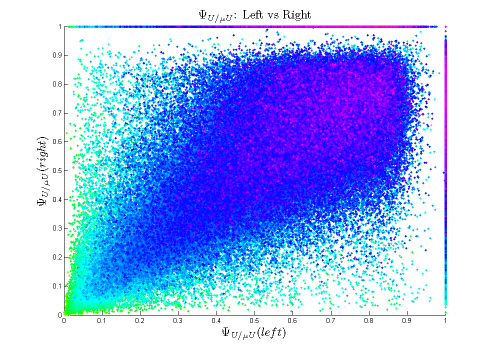
\includegraphics{fig4.png}

\section{Future Goals}
The following plan is for roughly the next two weeks.  There are two different paths for the project, and I plan to explore both simultaneously.  The visualizer will likely be sidelined for the rest of the project, unless something really needs to be visualized.
\subsection{BVH Building}
\begin{itemize}
\item Use real ray intersection data with my top-down analysis for several test scenes.  Produce graphs similar to the one above.
\item Extend the theoretical cost function to account for any-hit rays.
\item {\em Possible.} Find a way to test that a particular BVH is optimal.
\item {\em Possible.} Find a not-obviously-intractable method to interatively tweak the tree that will provably converge to an optimal tree.
\item {\em Possible.} Find tighter bounds for the minimum cost of a BVH over a set of leaves.
\end{itemize}
\subsection{BVH Traversal}
\begin{itemize}
\item For several test scenes, quantify the difference between RayOrder traversal and OrderedDepthFirst.  Identify, in terms of scene geometry, the cases in which they differ.  Consider incorporating the added cost of priority queue management into the cost metric for a BVH. 
\item Show the benefit (or lack thereof) of an {\em Almost Perfect Oracle} in traversing BVH trees for first-hit rays.
\item Fix the analysis package to handle any-hit rays.
\item Quantify the applicability of the Pareto principle for any-hit rays (a few subtrees intersect a large portions of the rays).
\end{itemize}
\end{document}